\documentclass{beamer}
\usetheme{Madrid} % professional, clean theme
\usepackage[utf8]{inputenc}
\usepackage{amsmath,amssymb}
\usepackage{graphicx}

\title{Burgers' Equation: Numerical Solution}
\author{Your Name}
\date{\today}

\begin{document}

% Title slide
\begin{frame}
\titlepage
\end{frame}

% Outline slide
\begin{frame}{Outline}
\tableofcontents
\end{frame}

% Introduction
\section{Introduction}
\begin{frame}{Burgers' Equation}
The one-dimensional Burgers' equation is a fundamental PDE given by:
\[
\frac{\partial u}{\partial t} + u \frac{\partial u}{\partial x} = \nu \frac{\partial^2 u}{\partial x^2},
\]
where:
\begin{itemize}
    \item $u(x,t)$ is the velocity field,
    \item $\nu$ is the kinematic viscosity,
    \item The first term represents nonlinear convection, and the second represents diffusion.
\end{itemize}
It is widely used as a simplified model for turbulence and shock formation.
\end{frame}

% Numerical Method
\section{Numerical Method}
\begin{frame}{Finite Difference Discretization}
Consider a uniform grid:
\[
x_0, x_1, \dots, x_N \quad \text{with spacing } \Delta x, \quad
t_0, t_1, \dots, t_M \quad \text{with step } \Delta t
\]

The explicit finite difference scheme is:
\[
u_i^{n+1} = u_i^n - \frac{\Delta t}{\Delta x} u_i^n (u_i^n - u_{i-1}^n) 
+ \nu \frac{\Delta t}{(\Delta x)^2} (u_{i+1}^n - 2 u_i^n + u_{i-1}^n)
\]

\begin{itemize}
    \item First term: nonlinear convection
    \item Second term: diffusion
    \item Simple explicit time-stepping
\end{itemize}
\end{frame}

% Example
\section{Example}
\begin{frame}{Initial and Boundary Conditions}
We solve on the domain $x \in [0,2]$ with:

\begin{itemize}
    \item Initial condition: $u(x,0) = -\sin(\pi x)$
    \item Boundary conditions: $u(0,t) = 0$, $u(2,t) = 0$
\end{itemize}

This setup allows us to observe shock formation and smoothing effects due to viscosity.
\end{frame}

\begin{frame}{Illustrative Results}
\begin{figure}[h]
\centering
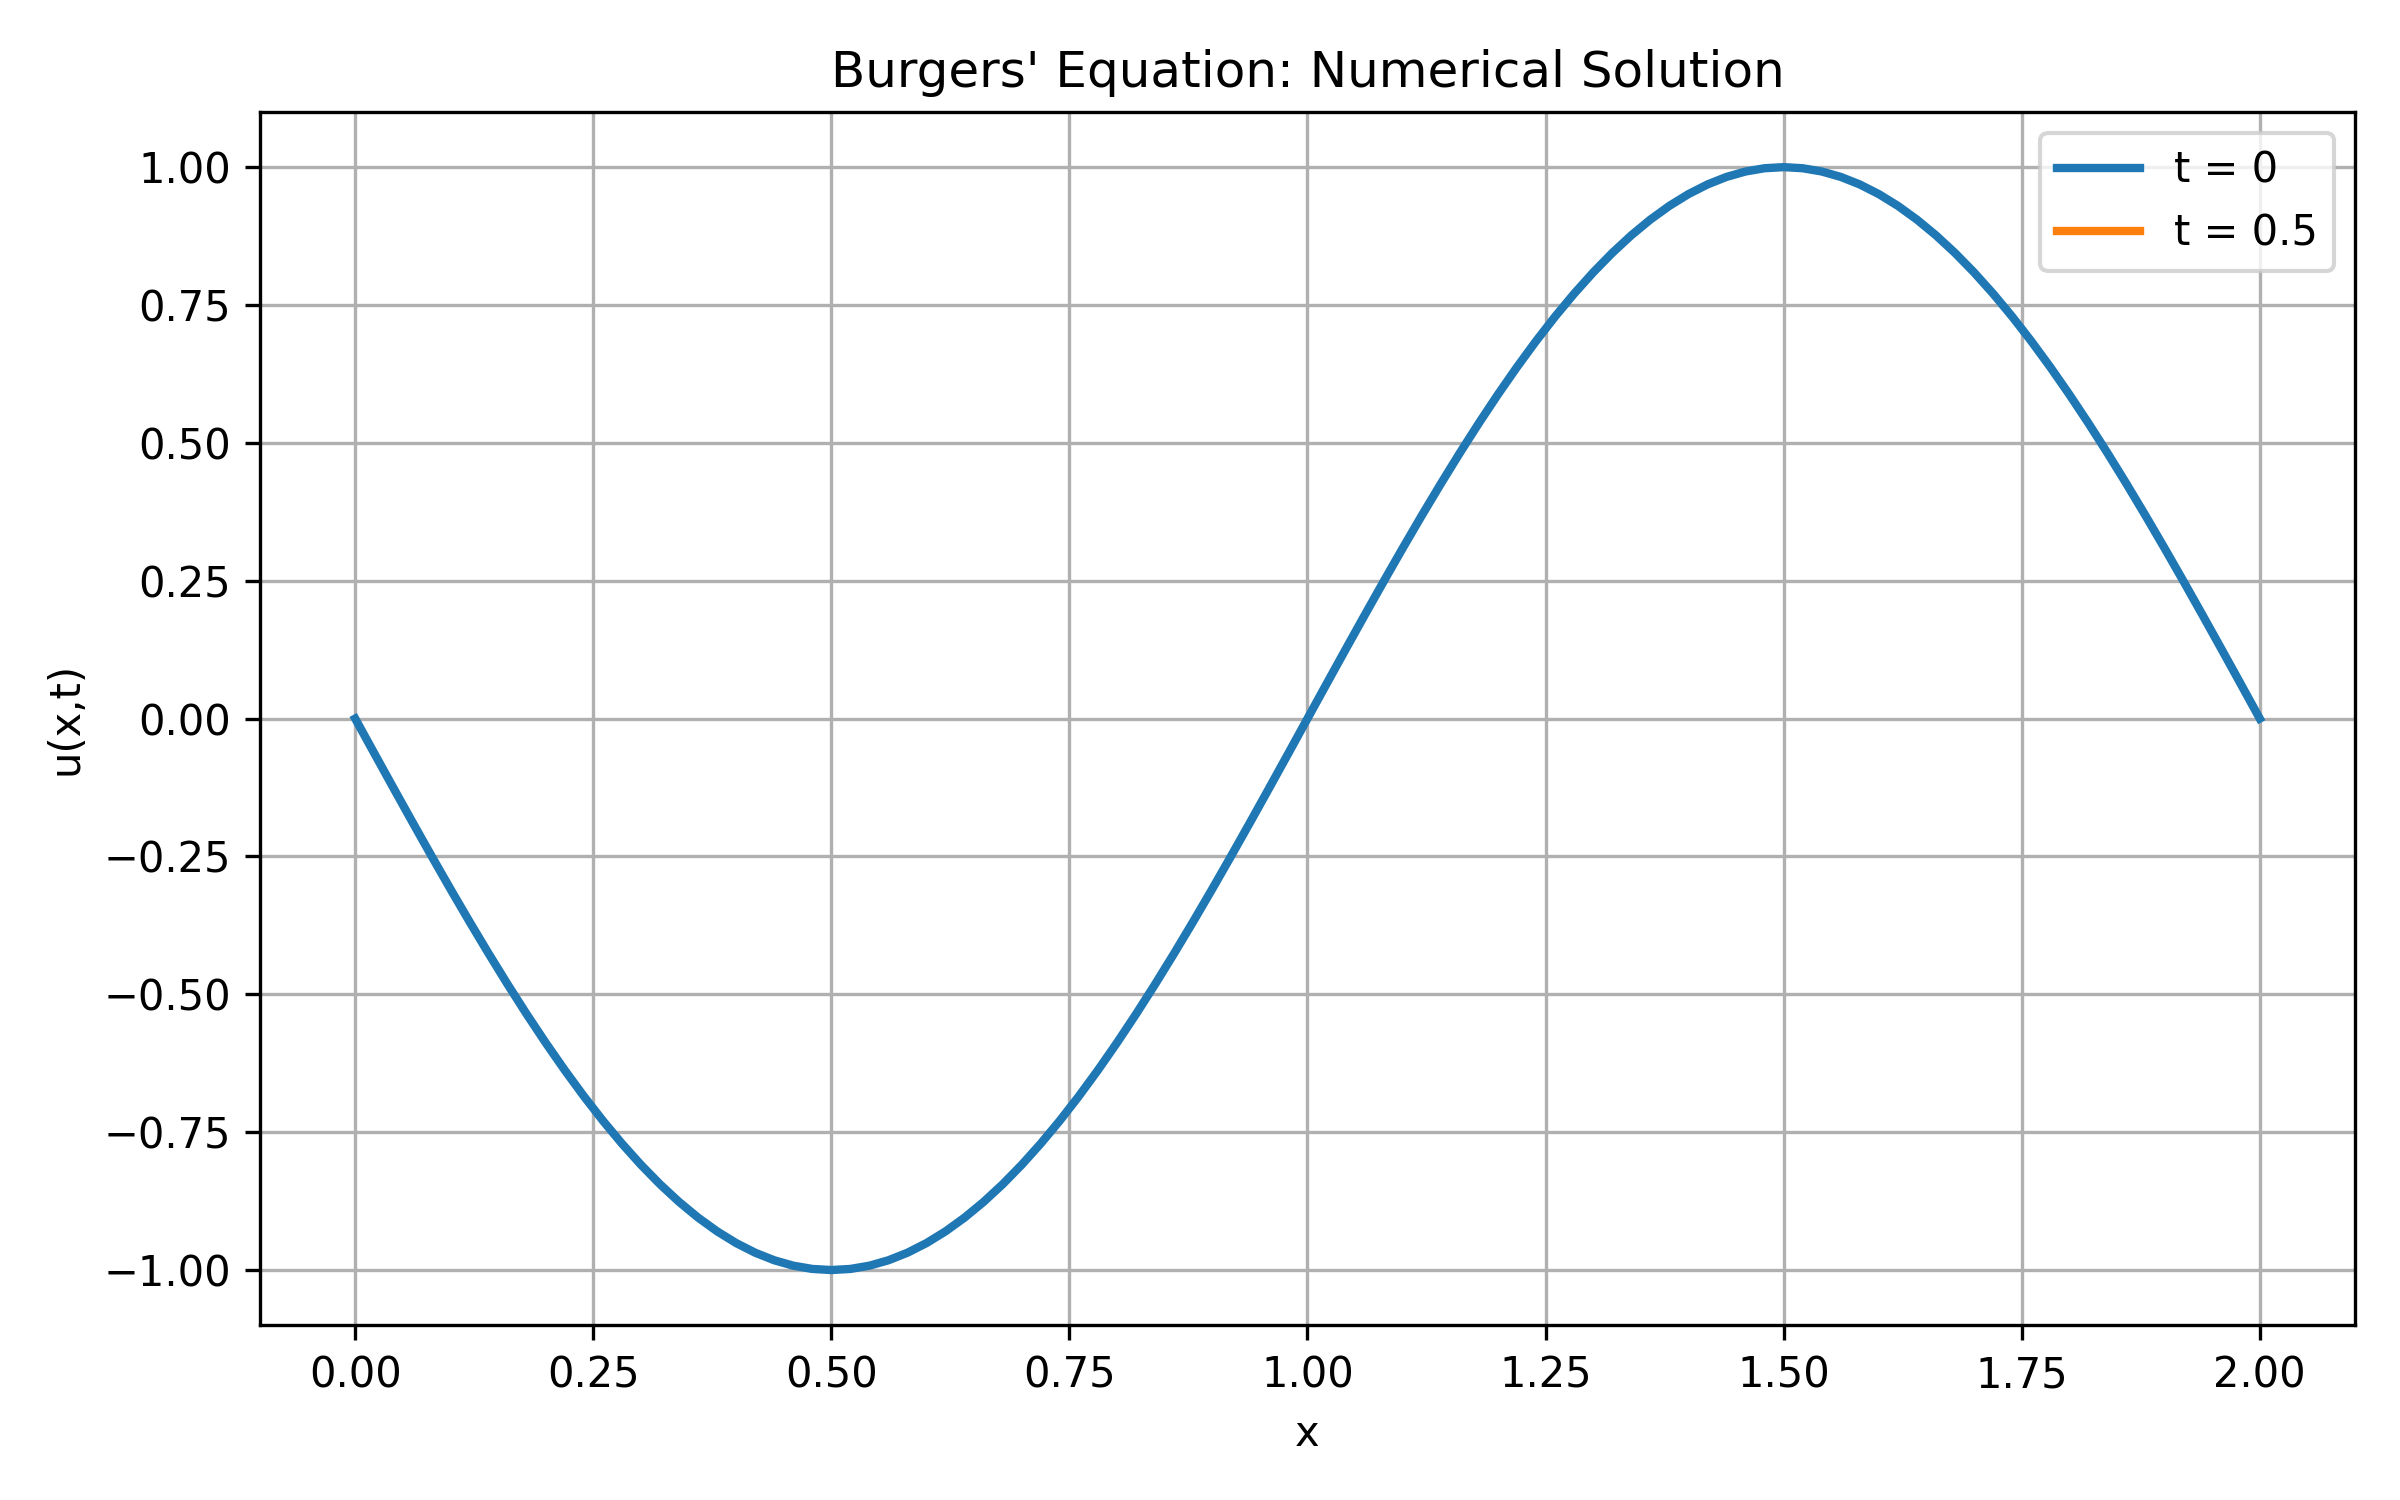
\includegraphics[width=0.8\linewidth]{burgers_plot.png} % replace with your figure
\caption{Numerical solution of Burgers' equation over time.}
\end{figure}
\end{frame}

% Discussion
\section{Discussion}
\begin{frame}{Observations}
\begin{itemize}
    \item Nonlinear convection leads to steep gradients (shock formation)
    \item Diffusion term smooths these gradients over time
    \item Stability requires careful choice of $\Delta t$ relative to $\Delta x$ (CFL condition)
    \item Burgers' equation is ideal for testing and understanding CFD solvers
\end{itemize}
\end{frame}

% Conclusion
\section{Conclusion}
\begin{frame}{Conclusion}
\begin{itemize}
    \item Burgers' equation demonstrates the interplay between convection and diffusion
    \item Numerical solutions illustrate shock formation and smoothing effects
    \item Serves as a foundational example for learning CFD methods
\end{itemize}
\end{frame}

\end{document}
